\chapter{Evaluation}

\paragraph*{}
The main purpose of the experiments executed for this thesis is to provide a better understanding of the practical feasibility of the solution for its stakeholders. The performance experiments are based on those of the paper \cite{LingZhen2021Sbtb} discussed in the background section. To be able to compare the results of this work and that of the paper, the experiments need to be made as similar as possible which will be clearly visible. Secondly, for the security evaluation the solution of this work will be evaluated and the differences with the security evaluation of \cite{LingZhen2021Sbtb} will be highlighted.

\section{Experiment setup}

\paragraph*{}
As was mentioned in the system model the experiments were not executed on the PinePhone itself, but on the QEMU emulator \cite{QEMU}. These emulations were run on a general-purpose laptop (Lenovo Thinkpad P50). The execution of the experiments themselves was rather straightforward. First, the emulation needed to be started, here all changed files were recompiled and the whole environment was put together. In the QEMU environment, we had to log in as root to enable the client application of the solution to access the necessary Linux files. When this was successful the solution had to be started, which was achieved in a similar way to how the OP-TEE example TAs are started up. This is because these examples were used as a source of inspiration, for how to put together a working OP-TEE application with TA (and PTA) interactions. 

\section{Performance}

\paragraph*{}
The trusted boot experiment in \cite{LingZhen2021Sbtb} is based on the attestation of the NW before giving it control. The paper states a performance of 107 MB of file system image being measured in 1.276 seconds. This could be a valuable starting point to compare with the performance achieved in this thesis. Because the implementation is focused on measuring code pages, there will be a difference in results. While it can be somehow assumed that the memory space of the file system in \cite{LingZhen2021Sbtb} is contiguous, or at least the mapping can be found rather easily, the code pages in the implementation of this work are spread across multiple processes which need to be considered one by one. Looking up the right memory pages to measure them incurs additional overhead which needs to be taken into account. That is why we opted for three different experiments that relate to this trusted boot experiment from \cite{LingZhen2021Sbtb}. One experiment will measure all the code pages of all the processes in the simulation, the second will measure all code pages of one process and the last experiment will measure one contiguous memory region of code pages from one process.

\paragraph*{}
The overhead of running the attestation module is measured in \cite{LingZhen2021Sbtb} by executing system services from the Linux kernel and running this experiment with and without the attestation module being active. The results in the paper of this experiment shows overhead between $- 0.55 \%$ and $+ 0.67 \%$ on different system calls. In our opinion, these results do not give much insight into the matter, because some key information is missing to correctly assess the results. First of all, it is not mentioned how often the attestation is running while these system calls are made. Secondly, it can be assumed that the attestation does not get priority over the system calls but this is also not explicitly mentioned. Last but not least, the range of $- 0.55 \%$ and $+ 0.67 \%$ does not really tell much, as this could just be standard deviation. For this experiment, it was not mentioned how often it was executed, which gives the impression that this is a one-time measurement. However, the authors of the paper are explicit about calling each service 1000 times, with intervals of 250 ms between each call, and they do this with 7 different system services, which, as they also include, adds up to almost 30 minutes.

\section{Performance Evaluation}

\paragraph*{}
The total amount of loaded code pages in RAM is around 1,850. The time it takes to measure these pages twice (once for initialization and once for attestation) is about 25 seconds. A plot is shown in figure \ref{graph} which provides the generated data points from the experiment being executed 10 times. Also a linear regression line can be found to provide the general correlation between the number of pages measured and the time it takes.

\begin{figure}[h!]
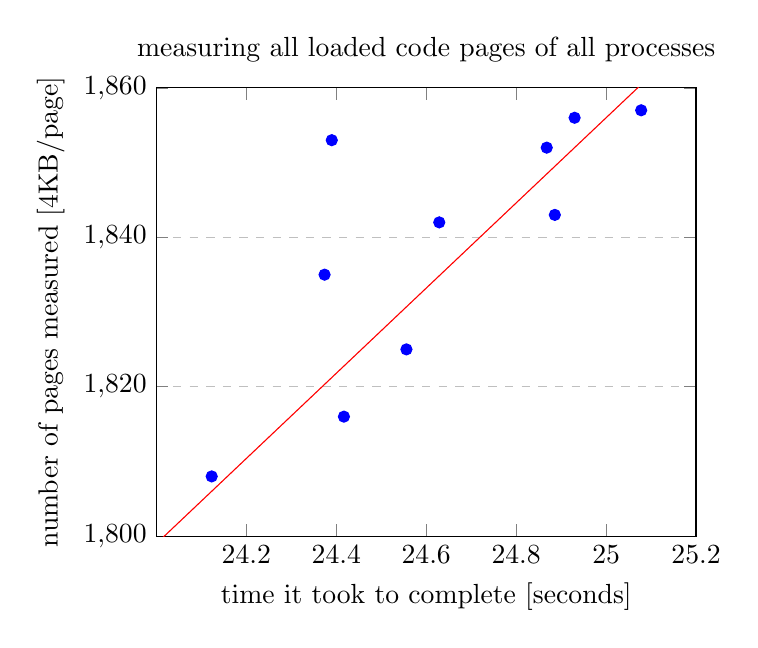
\begin{tikzpicture}
\begin{axis}[
    title={measuring all loaded code pages of all processes},
    xlabel={time it took to complete [seconds]},
    ylabel={number of pages measured [4KB/page]},
    xmin=24, xmax=25.2,
    ymin=1800, ymax=1860,
    xtick={24.2,24.4,24.6,24.8,25,25.2},
    ytick={1800,1820,1840,1860},
    legend pos=north west,
    ymajorgrids=true,
    grid style=dashed,
]

\addplot [
    domain=24:25.2, 
    samples=100, 
    color=red,
]{57*x + 431};

\addplot[
	only marks,
    color=blue,
    mark=*,
    ]
    coordinates {
    (24.868,1852)(24.886,1843)(24.556,1825)(24.930,1856)(24.390,1853)(24.123,1808)(24.417,1816)(24.629,1842)(25.078,1857)(24.374,1835)
    };
    
\end{axis}
\end{tikzpicture}
\caption{Measurement plot for all processes}
\label{graph}
\end{figure}

\paragraph*{}
To provide insight into how long it takes to measure one process (twice), the last experiment was executed on the \textit{init\_proc} process. The results of this experiment can be seen in figure \ref{init}.

\begin{figure}[h!]
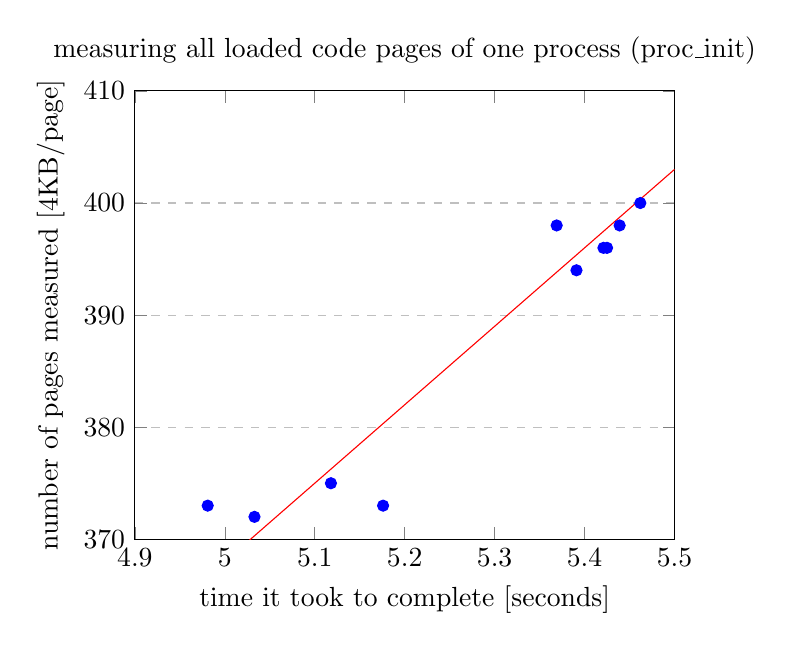
\begin{tikzpicture}
\begin{axis}[
    title={measuring all loaded code pages of one process (proc\_init)},
    xlabel={time it took to complete [seconds]},
    ylabel={number of pages measured [4KB/page]},
    xmin=4.9, xmax=5.5,
    ymin=370, ymax=410,
    xtick={4.9,5,5.1,5.2,5.3,5.4,5.5},
    ytick={370,380,390,400,410},
    legend pos=north west,
    ymajorgrids=true,
    grid style=dashed,
]

\addplot [
    domain=4.9:5.5, 
    samples=100, 
    color=red,
]{70*x + 18};

\addplot[
	only marks,
    color=blue,
    mark=*,
    ]
    coordinates {
    (4.981,373)(5.421,396)(5.369,398)(5.462,400)(5.391,394)(5.033,372)(5.439,398)(5.425,396)(5.118,375)(5.176,373)
    };
    
\end{axis}
\end{tikzpicture}
\caption{Measurement plot for one process}
\label{init}
\end{figure}

\paragraph*{}
In the first two experiments the amount of pages that are loaded into RAM fluctuates a bit. Which probably has to do with pages being swapped in and out of memory. In this last experiment, only one executable memory region of the \textit{init\_proc} is measured and the amount of pages stays constant for all 10 iterations. The amount of pages measured is 88 and the average execution time is 1.319 seconds, the maximum execution time is 1.353, and the minimum 1.299.

\paragraph*{}
Last but not least, the three experiments are plotted in one graph in figure \ref{last} to show how they relate to each other. The mean values of every experiment have been taken to fit each experiment in one data point. They would be very close to one another anyway. This plot clearly shows that the amount of time the measurements take is proportional to the number of pages that are measured. The reason for this is that hashing the memory pages is the most compute-intensive task of the program, and the file overhead is similar, because for every process two files need to be read. This graph allows us to compare the performance of our experiments to that of \cite{LingZhen2021Sbtb}, because we can extrapolate the results to the necessary amount of pages that were measured in the paper. In the paper, 107 MB (of file system image) was measured in 1.276 seconds. We achieve a similar execution time for only 88 executable pages. As explained these were measured twice: once for the initialization phase and once during the attestation phase. This comes down to 352 KB measured twice or 704 KB, which is less than 1\% of their measured memory. If we extrapolate based on the number of pages, it is best to start from the largest experiment to have the least rounding errors. The mean of this first experiment comes down to 1,839 pages measured in 24.625 seconds, 107 MB equals 26 750 pages. Measuring this many pages would require our implementation a little less than 360 seconds or 6 minutes. 

\begin{figure}[h!]
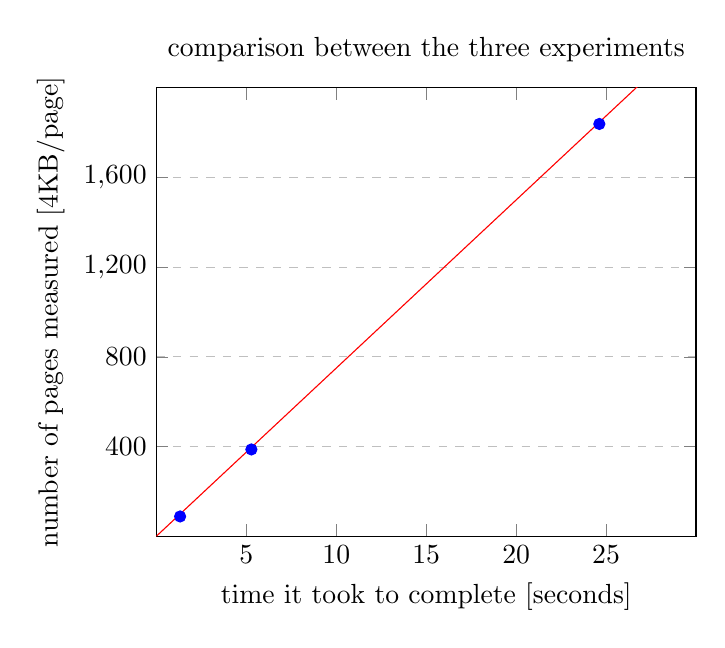
\begin{tikzpicture}
\begin{axis}[
    title={comparison between the three experiments},
    xlabel={time it took to complete [seconds]},
    ylabel={number of pages measured [4KB/page]},
    xmin=0, xmax=30,
    ymin=0, ymax=2000,
    xtick={5,10,15,20,25},
    ytick={400,800,1200,1600},
    legend pos=north west,
    ymajorgrids=true,
    grid style=dashed,
]

\addplot [
    domain=0:30, 
    samples=100, 
    color=red,
]{75*x};

\addplot[
	only marks,
    color=blue,
    mark=*,
    ]
    coordinates {
    (24.625,1839)(5.281,387)(1.319,88)
    };
    
\end{axis}
\end{tikzpicture}
\caption{Comparison of the three measurement experiments}
\label{last}
\end{figure}

\paragraph*{}
As can be seen in the three executed experiments, the performance of the implementation of this work differs a lot from that of \cite{LingZhen2021Sbtb}. Some aspects need some explaining, however. First of all, the implementation is not written nor fine-tuned for performance, it is merely written as a proof of concept. This is due to the memory regions that are attested in this work being only the executable memory pages of a process. These pages need to be identified using multiple files, which generally takes more time compared to the case with one large chunk of memory that is attested. It is also important to take into account that executable pages take up less memory than a file system would generally do. Lastly, these experiments are executed on a Qemu emulation of OP-TEE on a general-purpose laptop (Lenovo Thinkpad P50), while the experiments in \cite{LingZhen2021Sbtb} are executed using a hardware prototype. 

\paragraph*{}
A good balance between performance overhead and security assurance depends on the use case. In the case of a smartphone, we believe even with these results that attesting the executable pages that are loaded in RAM every 30 minutes has not too much impact on the user experience. Depending on the amount of newly loaded memory pages when an application is started, it could even be considered to attest these pages before starting to execute them. This could impact the user experience much more because this happens while the user is waiting for the application to open. While on the other hand, running the attestation in the background on the already loaded pages in RAM, should have minimal impact on the user. These considerations do not take into account the energy consumption of running the attestation, because we didn't have the means for these kinds of experiments.

\section{Security Properties}

\paragraph*{}
The attestation method presented in this work focuses on measuring the code pages of processes loaded in RAM. A code page can only gain control or be executed when it is loaded in RAM first. Keeping this prerequisite in mind, it should suffice to only attest those pages to ensure no corrupted code page gets executed. To put it more mildly, the measurements should run periodically, so a code page may have been executed before the changes are noticed by the attestation PTA.

\paragraph*{}
The integrity of the measurement execution is of utmost importance when it comes to attestation. In RA, the critical code runs on a hardened server, which guarantees that it is infeasible to tamper with the execution control flow. In the case of the PinePhone, the RA method is not used. Instead, user-controlled attestation is applied, which allows the user to verify the trustworthiness of his device. The critical code which compares the measurements runs in the SW. The TEE provided by ARM TrustZone does guarantee that the NW cannot influence the execution of the SW in any way, as long as the device was started up successfully using secure boot.

\paragraph*{}
Secure storage of results is very important for a liable attestation method. If an adversary were able to tamper with these values, they could make every attestation attempt fail due to the changed initial value. In case a bad hashing algorithm is chosen and the attacker can read the initial hash digest, he could also try to forge a collision attack \cite{SafaryanOlga2021MHCC} where he tampers with a page in such a way that its hash digest does not change but the code in the page does something the attacker desires. To make sure the reference values are not tampered with, they need to be stored in secure memory which should not be accessible from outside the SW. In the SW, these values should only be written during the initialization phase and afterward only read. This needs to be stated less strictly. In case there are software updates or additional software to be installed on the device, the initial values will have to be overwritten. The initialization phase could be executed again to update or add the measurement results for those code pages. 

\section{Security Evaluation}

\paragraph*{}
Security guarantees that can be made, are the integrity of the measurement execution control flow and the integrity and confidentiality of the results that are being stored. These are achieved thanks to secure boot process enabling the TEE of ARM TrustZone. These are key assumptions in the field of RA, and thus are also very important in this case of user-controlled attestation. Of course, when discussing the security guarantees of a certain solution, it is not only about the execution and storage of the measuring application itself, but also about what additional security guarantees it provides to the system overall. The most important guarantee that an attestation solution tries to provide, is being able to detect modifications or unexpected possibly malicious changes to the aspects of the system it attests. In our case, the code pages of processes are being attested, we only measure the ones that are present in RAM, because only then they are able to harm the system. As stated in \cite{LingZhen2021Sbtb} there is still an unsolved problem, the rich OS needs to provide the physical addresses of the code pages. This means that malware capable of self hiding or transient rootkits are still possible threats that could stay unnoticed by this solution. If an adversary has taken control of the OS, there are countless ways in which the attacker could deny the attestation PTA to obtain the necessary addresses, which would be very hard to identify and alert the user.

\paragraph*{}
OS/firmware attacks are present in the attacker model of \cite{LingZhen2021Sbtb} on which this work is based. We believe that with this method the code pages of all processes, including those of the rich OS, can be attested and this will enable the user to be notified about any tampering with this code base. This does not mean, however, that tampering with these code pages has become harder. Besides tampering with code, there are also lots of different methods to perform an OS/firmware attack. We believe that this work can be extended to thoroughly attest the NW, but in its current state it only allows detection of a small portion of the OS/firmware attack surface.

\paragraph*{}
It is also claimed by \cite{LingZhen2021Sbtb} that software attacks are protected against or detectable in the case of attestation. Again, with their addendum about only securing the code section of processes, this is valid but the integrity of the code is only a small portion of the attack surface. In their measurement method, the data structures are not checked, and those are the main target for very well-known attacks that have been around for decades, like buffer overflows and return-oriented programming. Extensions to this solution need to be realized to detect software attacks, OS/firmware attacks likewise.